\chapter{Overview of the hardware}

\section{Features of the DE10-Nano development board}

On the board, numerous devices are made available to the user. Some of them will be very 
interesting for this work: the Cyclone V FPGA (A in Figure \ref{fig:de10/de10_features}) that is
basically the main component of the system as almost everything on the board is driven by it. It is
also where all the hardware designed in the work resides. The 1GB DDR3 RAM (B) which is used 
by the ARM side of the FPGA. An ethernet port (C) which can be
useful to connect to the ARM processor from any external environment. For instance, SSH can be used
to connect to it if the installed system can handle it. Then there are the SD card reader and the SD 
card (D, on the other side of the PCB). The SD card consists in the mass storage of this board. The
one used offers 8GB of memory. Another important component is the HDMI output (E) that can be used
from the programmable logic. Other less important devices, mainly IOs are avaible: General Purpose 
Input / Output pins (GPIOs), LEDs, buttons and switches. All of these devices are discussed at some
point in this report. The ones that are not listed (such as the IMU system) haven't been used.

\begin{figure}[ht]
    \centering
    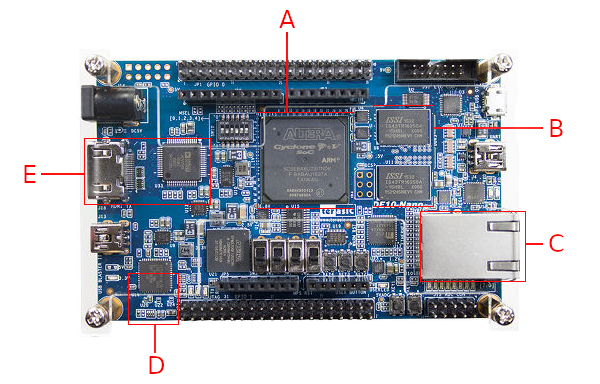
\includegraphics[scale=0.6]{Chapter1-Hardware/res/de10_nano.png}
    \caption{DE10 Nano development board main features}
    \label{fig:de10/de10_features}
\end{figure}

\section{Programmable logic devices}

Field Programmable Gate Arrays (FPGAs) are a type of Programmable Logic Device (PLD) which are, as 
the name suggests, programmable logic circuits. Programmable means that the user can choose which 
circuitry will be implemented in these devices and as it will be shown in this chapter, some of 
these devices are very versatile! They can implement almost any kind of digital circuit.

PLDs come in different forms but follow a similar pattern for most types. In fact, they almost all 
are composed of an AND array and an OR array that are both programmable or not. Here, a discussion 
of these different types and their evolution will be made to arrive at FPGAs and show the advantages 
and disadvantages compared to other technologies.

\subsection{ROM based PLDs}

This first type is very simple, as shown in Figure \ref{fig:fpga/pld_rom_external}. In fact, the 
circuit, which can only be combinatorial, will be simulated by a ROM. Each address corresponds to 
an input of the circuit and each word in memory to an output of the circuit. The ROM therefore 
simply contains the truth table of the logic circuit to be implemented.

\begin{figure}[ht]
    \centering
    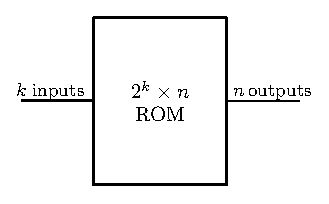
\includegraphics[scale=1.2]{Chapter1-Hardware/res/pld_rom_external}
    \caption{An external view of ROM based PLDs}
    \label{fig:fpga/pld_rom_external}
\end{figure}

The inside of a $2^2 \times 4$ ROM can be seen as a 2-to-4 decoder followed with a 4-by-4 OR gates 
array where the connections in the array are configurable. They can be opened or closed during the
programmation of the device. The decoder can be interpreted as the AND gates array here. Thus, the
AND gates array is fixed and the OR gates array is programmable for this kind of devices.

An example corresponding to the $2^2 \times 4$ ROM is given in Figure \ref{fig:fpga/pld_rom_internal}.
In this example, the array is represented by a grid. All horizontal lines represent a 1-bit signal
that can be connected to an OR gate. The signal is connected if a red x is present at the connection
point. As can be seen, the OR gates array is here programmed to describe the truth tables of these 
boolean equations

\begin{equation*}
    \begin{cases}
        A_0& = I_0 \cdot \bar{I_1} \\
        A_1& = \bar{I_1} \\
        A_2& = 0 \\
        A_3& = \bar{I_0} \cdot I_1
    \end{cases}
\end{equation*}

Obviously, real devices contain a lot more signals and gates to be cost effective and useful. 
As stated previously, the ROM PLDs can only represent combinatorial circuits. There is no register
or feedback loop in the circuits that are described with this technology.

\begin{figure}[ht]
    \centering
    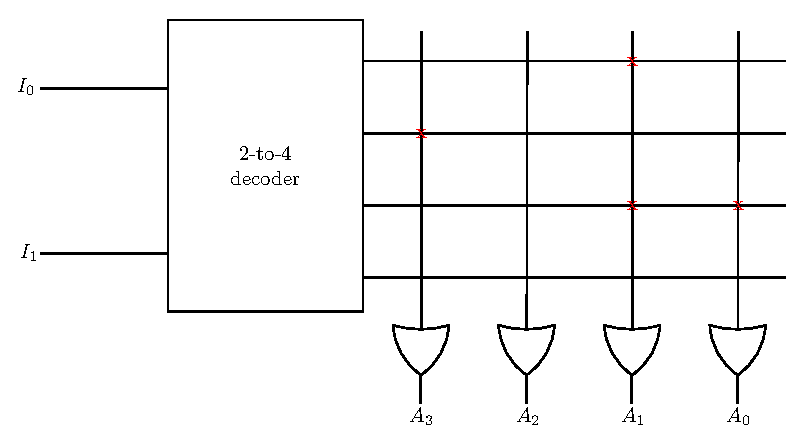
\includegraphics[scale=0.8]{Chapter1-Hardware/res/pld_rom_internal}
    \caption{An internal view of ROM based PLDs}
    \label{fig:fpga/pld_rom_internal}
\end{figure}

\subsection{PAL and PLA}

The Programmable Array Logic (PAL) and Programmable Logic Array (PLA) devices differ from the ROM 
based PLDs as they both have a programmable AND gates array. However, only the PLAs have bot AND and
OR gates arrays that are programmable. The PLAs are thus the most flexible devices of the three.
As expected, this flexibility makes them also more complex and complicated to program. The outputs
of these devices can often be complemented through programmation too. It should also be notticed
that both the inputs and the inverted inputs are directly available in the arrays here, as visible
in Figure \ref{fig:fpga/pld_pla_internal}. These small additions greatly increase the possibilities
of such devices as programmable logic wont be used for that purpose.

\begin{figure}[ht]
    \centering
    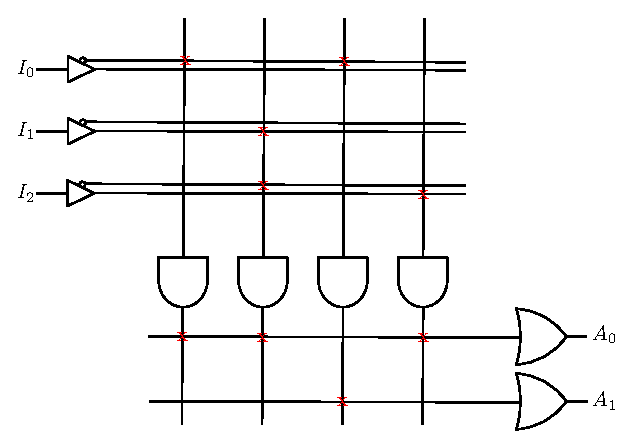
\includegraphics[scale=0.8]{Chapter1-Hardware/res/pld_pla}
    \caption{An internal view of PLAs}
    \label{fig:fpga/pld_pla_internal}
\end{figure}

\subsection{Programming methods}

It is very interesting to have programmable devices but it is even better when one can program them 
so this section contains a brief discussion of the common different programming techniques.
 
Initially, these devices were mainly programmable in two ways. The first was to use fuses and 
anti-fuses at each interconnection. The user then had to apply destructive currents to the right 
places for the fuses to open the connections and the anti-fuses to close them. The second method was 
to leave it to the user to complete the IC design. One would then make a mask to select which 
interconnects to open and close. To provide some examples, the fuse methods are used in PROMs and 
masks for ROM based PLDs. Both of these programming methods make the devices non-erasable, which at 
the same time makes them non-reprogrammable. However, they are both non-volatile which can be an 
advantage when the user don't want any boot latency at startup.

Later, other programming techniques were developed following the emergence of transistors. Indeed, 
these transistors are placed at the interconnections and controlled by their gate with the help of 
a bit kept in a memory. The memory can then be programmed to define the behaviour of the connections 
without them being frozen forever. As the memory is usually SRAM, the devices become reprogrammable
but still volatile. Other technologies have subsequently made it possible to have non-volatile 
memory in addition to memory by using, for example, floating gate transistors. These two types of 
interconnections are usually configured by applying a high current to set or reset the memory state. 

\section{The case of FPGAs}

Now that an introduction to PLDs and programming methods has been made, it is time to get to the 
heart of the matter with a description of FPGAs. In this section, it will be tried to be general 
enough to cover the operation of a large number of FPGAs. More details will be given in the next 
section when it will be about the FPGA used for the realization of this thesis.

FPGAs are fascinating yet complex devices. Indeed, they have three main programmable levels. These 
three levels will be discussed in turn, starting with the programmable logic blocks, then the 
programmable interconnect and finally the programmable I/Os. 

\subsection{Programmable logic blocks}

Programmable blocks are present in very large numbers in modern FPGAs (commonly tens to hundreds of 
thousands). They are the basic elements of the circuits implemented on FPGAs. Due to their 
architecture, which can be seen in Figure \ref{fig:fpga/fpga_block}, they allow both combinational 
and sequential circuits to be implemented. 

\begin{figure}[ht]
    \centering
    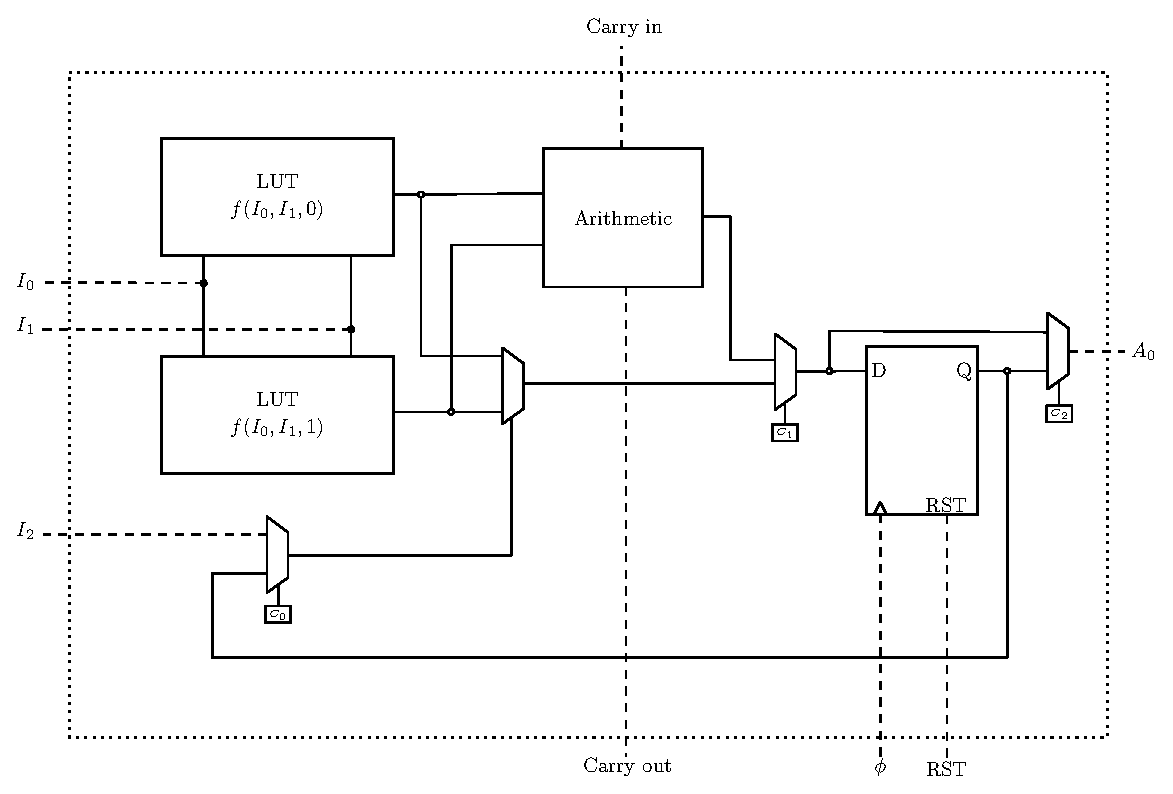
\includegraphics[scale=0.8]{Chapter1-Hardware/res/fpga_block}
    \caption{An FPGA programmable logic block}
    \label{fig:fpga/fpga_block}
\end{figure}

The combinatorial part of the circuits is implemented using a LookUp Table (LUT). The truth table is 
simply stored in this LUT as for the ROM PLDs but the bits are now stored in SRAM. If one LUT is 
not sufficient, the logic function can be implemented on several LUTs connected at the output by a 
multiplexer that is controlled by the remaining inputs. This is made fully valid by Shannon's 
expansion theorem. 

\begin{theorem}
    Any boolean function $f(x_1, x_2, ..., x_n)$ can be expressed as 
    \begin{equation*}
        f(x_1, x_2, ..., x_n) = x_n \cdot f(x_1, x_2, ..., x_{n - 1}, 1) + \bar{x_n} \cdot 
        f(x_1, x_2, ..., x_{n - 1}, 0)
    \end{equation*}
\end{theorem}

As shown in Figure \ref{fig:fpga/fpga_block}, the blocks also have an arithmetic sub-block and a 
register. Having this arithmetic block in each single programmable block greatly increases the 
efficiency of the FPGAs and reduces the latency of the blocks, even if sometimes these circuits are 
simple carry adders. Fixed hardware is always faster than programmable one as they are better 
optimized. In addition to the programmable LUTs, other configuration bits are available to control
the behaviour of the multiplexers: $C_1$, $C_2$ and $C_3$ allowing respectively to add a feedback 
loop to the block, to select the result of the boolean function or that of the arithmetic sub-block 
and to make the output of the block registered or not.

In brief, these blocks are the heart of the FPGA. All their features and configuration bits allow 
them to describe almost any kind of digital circuit in an efficient way.

\subsection{Non-programmable blocks}

Other non-programmable or less programmable blocks are also available on the FPGA. They are divided 
into two main groups: memories and utilities. Memories are simply blocks that can store data. A 
specific discussion of these memory blocks will be made in a later section. On the utility side, 
there can be a wide variety of blocks: multipliers, PLLs, DSPs and even whole CPUs. In short, 
enough to make FPGAs even more powerful!

\subsection{Programmable interconnect}

Programmable blocks are very versatile and efficient, but they need to be connected to each other to 
make large circuits. As can be seen in Figure \ref{fig:fpga/fpga_interconnect}, the blocks are 
positioned on a grid and the interconnection passes around them. 

\begin{figure}[ht]
    \centering
    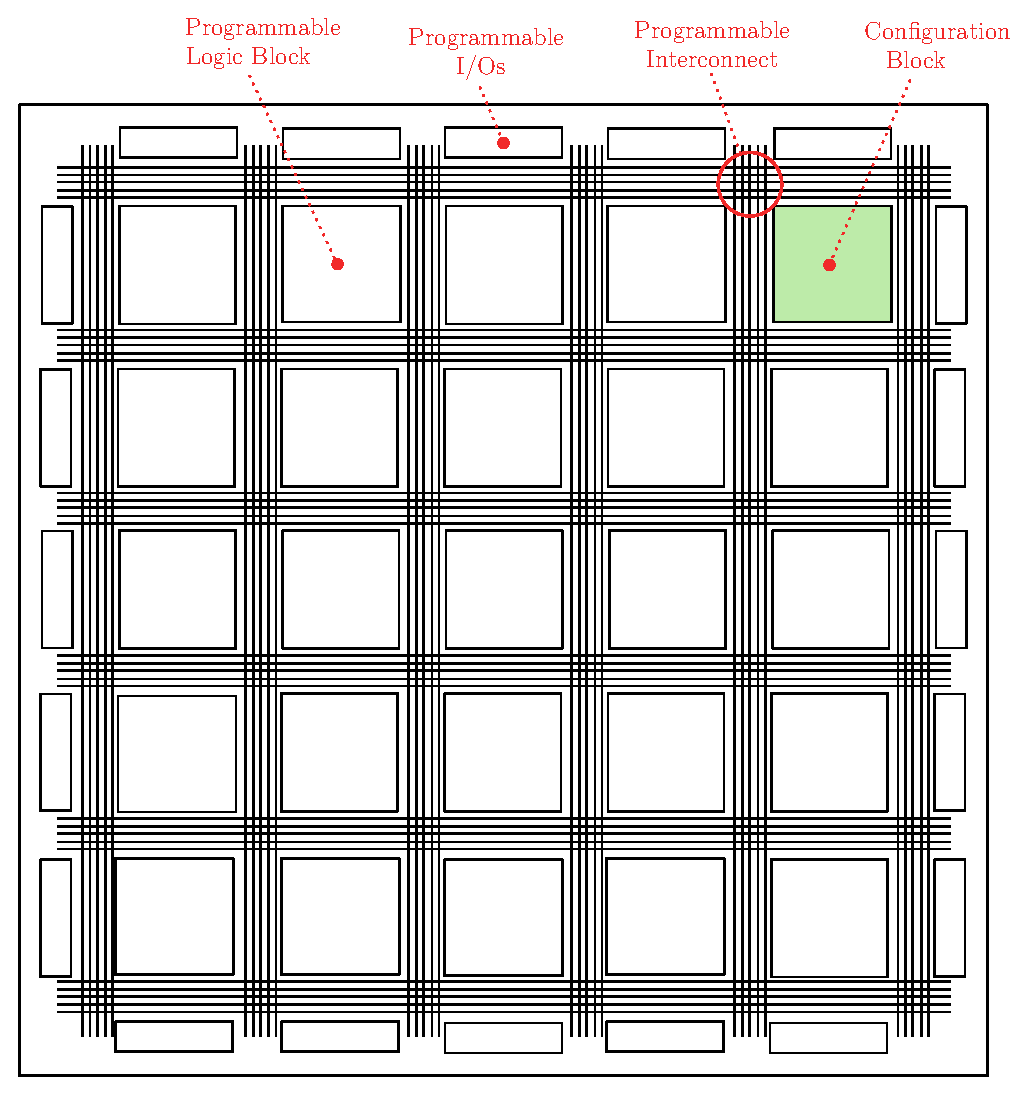
\includegraphics[scale=0.6]{Chapter1-Hardware/res/fpga_interconnect}
    \caption{High level view of an FPGA}
    \label{fig:fpga/fpga_interconnect}
\end{figure}

For this purpose, there is the programmable interconnection that will allow the signals to be routed 
from one block to another. To do this, configurable switches are placed at the crossings of the 
tracks. However, everything must be connected, whether the blocks are close or distant. As this 
cannot be done directly without causing problems in terms of time and power constraints, several 
hierarchical connection levels are present. However, in order to keep the explanations simple, it 
will be considered here that there is only one level. It should also be noted that each switch adds 
latency to the signal, so the interconnection is optimised to limit the number of switches between 
blocks. 

In addition to this configurable interconnection, there are also tracks to bring global signals 
everywhere. Among these signals are the clock, the resets, ... On a more local level, some signals 
are also shared between the blocks. These include, for example, the carry signals of the arithmetic 
sub-blocks.

\subsection{Programmable I/Os}

Now that almost the entire interior of the FPGA has been described, all that remains is to connect 
it to the outside. This is why there are these I/O pins all around the FPGA in Figure 
\ref{fig:fpga/fpga_interconnect}. These as well as the other parts of the FPGA are also 
configurable. As it is desirable for the FPGA to adapt to a wide variety of external hardware, these 
pins can be configured to the standard used. They can also be used as input, output, bi-directional, 
differential pairs, ... In short, they allow a large number of configurations so that the designed 
circuit can be adapted and coupled with a maximum of other circuits.

\subsection{Programmation of the FPGA}

Due to their complexity, the configuration circuitry of the FPGA is just as complex. For this 
reason, few details will be provided in this section. That said, it should be noted that part of 
the FPGA is assigned to this function. This block will then take care of configuring all the 
configuration bits in the relevant memories. However, since the memories holding the configuration 
within the FPGA are volatile, it will often be necessary to couple a non-volatile memory to the 
FPGA to retain its configuration. The configuration will therefore have to be re-configured each 
time the FPGA is rebooted, which can create some latency. It is also important to note that the 
memory holding the configuration must be relatively large, as the number of configuration bits is 
very large. More details on compiling designs and configuring FPGAs in practice will be given in a 
later section.

This closes the theoretical discussion on FPGAs. As repeated several times, FPGAs are extremely 
powerful and configurable. This allows them to describe a large number of circuits and to adapt to
many existing circuits. Another advantage is that they are massively parallel due to their 
structure. A user can implement twenty different circuits running in parallel. Despite all these 
advantages, FPGAs still have some drawbacks. One of them is cost. Some FPGAs can cost several 
thousand euros. The complexity and difficulty of access is another problem for designers, the 
datasheets are numerous and extremely long, the tools are also numerous and not always easy to use. 
Electrical power requirements and start-up latency are also two other factors that must be taken 
into account when a user chooses an FPGA for circuit development. Nothing is perfect, not even 
FPGAs.

\section{Inside Cyclone V}

\subsection{Programmable logic side}

\subsection{ARM processor side}

\subsection{Cyclone V interconnect}

\section{Board memories comparison}